\documentclass{beamer}

\mode<presentation>
{
  \usetheme{Goettingen}
  \usecolortheme{seahorse}
  \setbeamercovered{transparent}
}

\usepackage[english]{babel}
\usepackage[latin1]{inputenc}

\usepackage{graphicx}
\graphicspath{ {images/} }

\usepackage{times}
\usepackage[T1]{fontenc}

\setlength{\parskip}{1em}

\title{When is a\\ crystal graph\\ not\\ crystallographic?}

\author[Olaf Delgado]{Olaf Delgado-Friedrichs}

\date{Order!Order? --- Canberra 4 Dec 2019}

\begin{document}

\begin{frame}
  \titlepage
\end{frame}


\section{Too much symmetry}

\begin{frame}
  \begin{center}
    Answer: when it has ``too much symmetry''.

    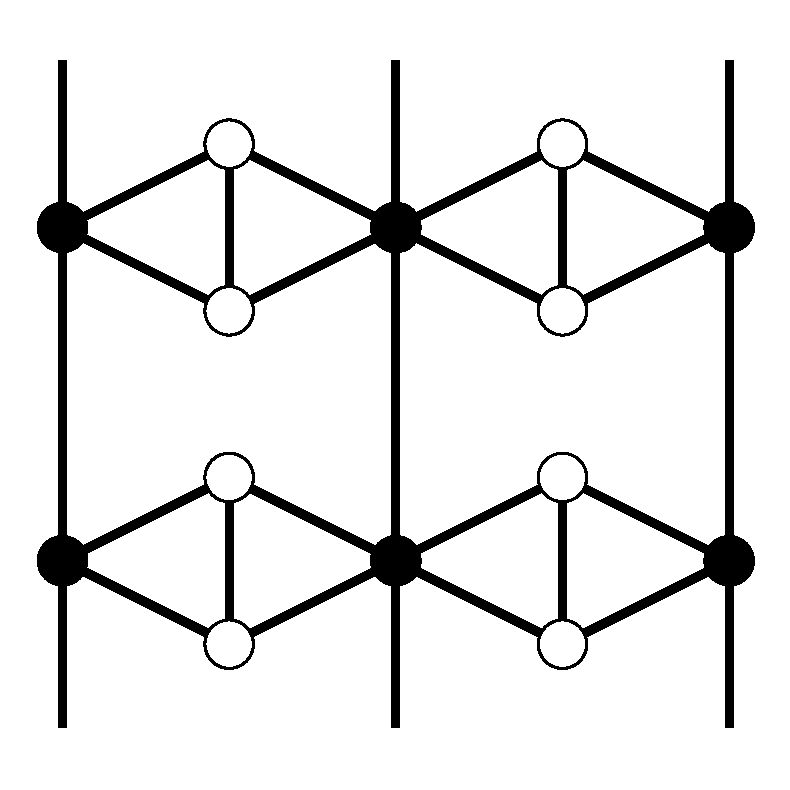
\includegraphics[width=1.7in]{unstable}
    \qquad
    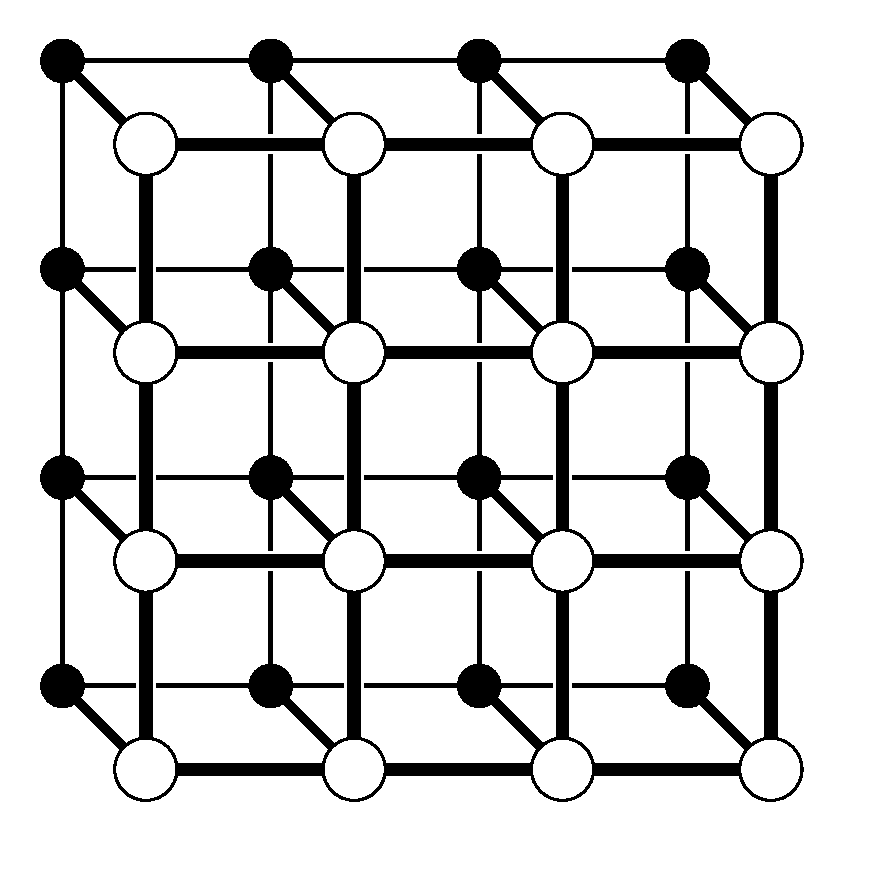
\includegraphics[width=1.7in]{ladder}

    More precisely: when its automorphism group is not a crystallographic
    space group.

    ({\em Crystallographic nets and their quotient graphs,}\\
    W.\ E.\ Klee 2004.)
  \end{center}
\end{frame}


\section{Crystal nets}

\begin{frame}
  \begin{center}
    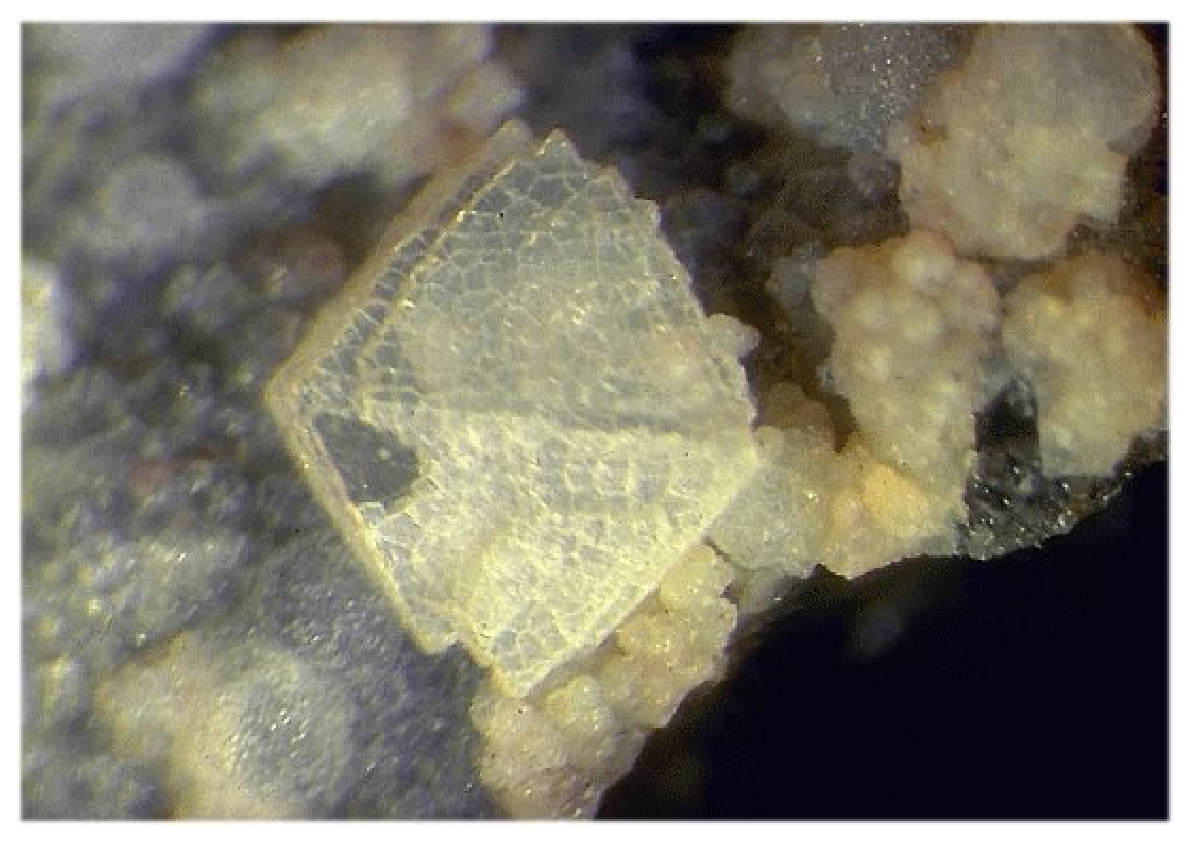
\includegraphics[height=2.5in]{fau-photo}

    A crystalline material.  What might be its atomic structure?
  \end{center}
\end{frame}

\begin{frame}
  \begin{center}
    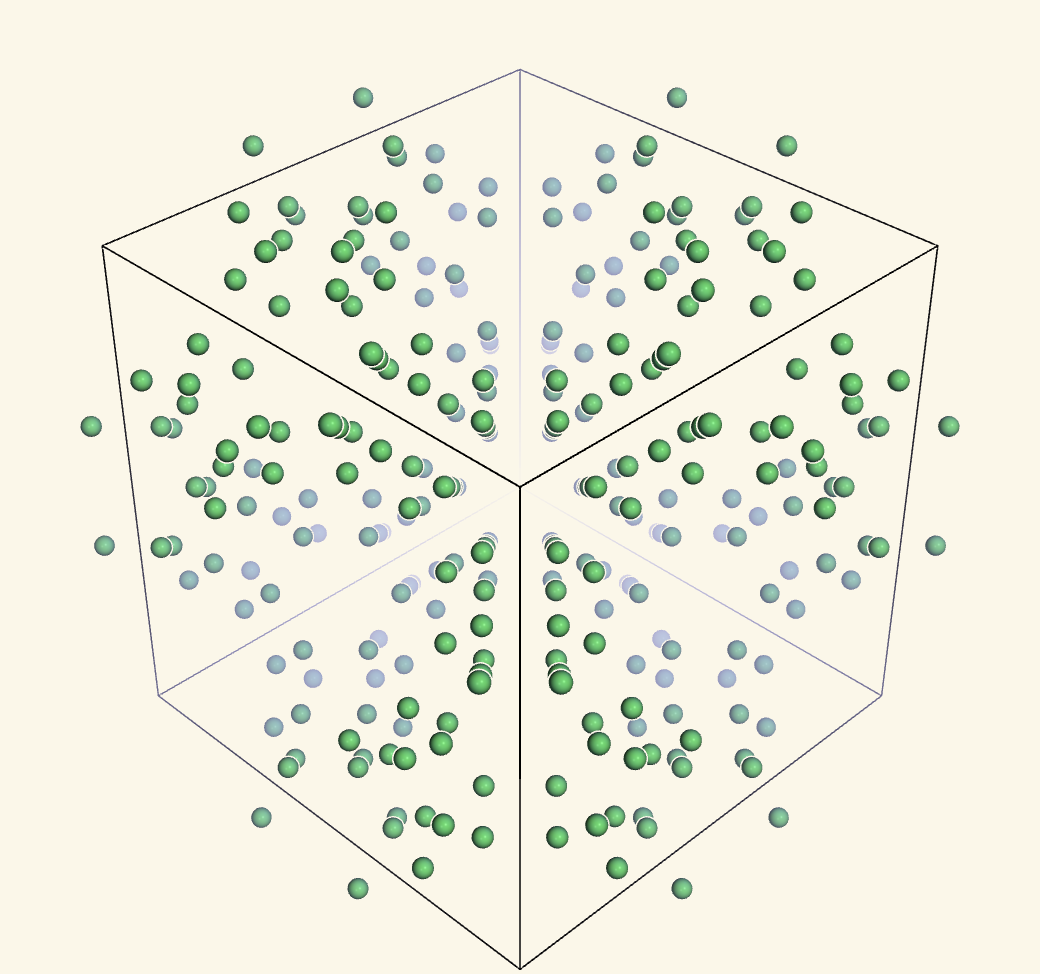
\includegraphics[height=3in]{fau-atoms-new}

    X-ray crystallography produces something like this.
  \end{center}
\end{frame}

\begin{frame}
  \begin{center}
    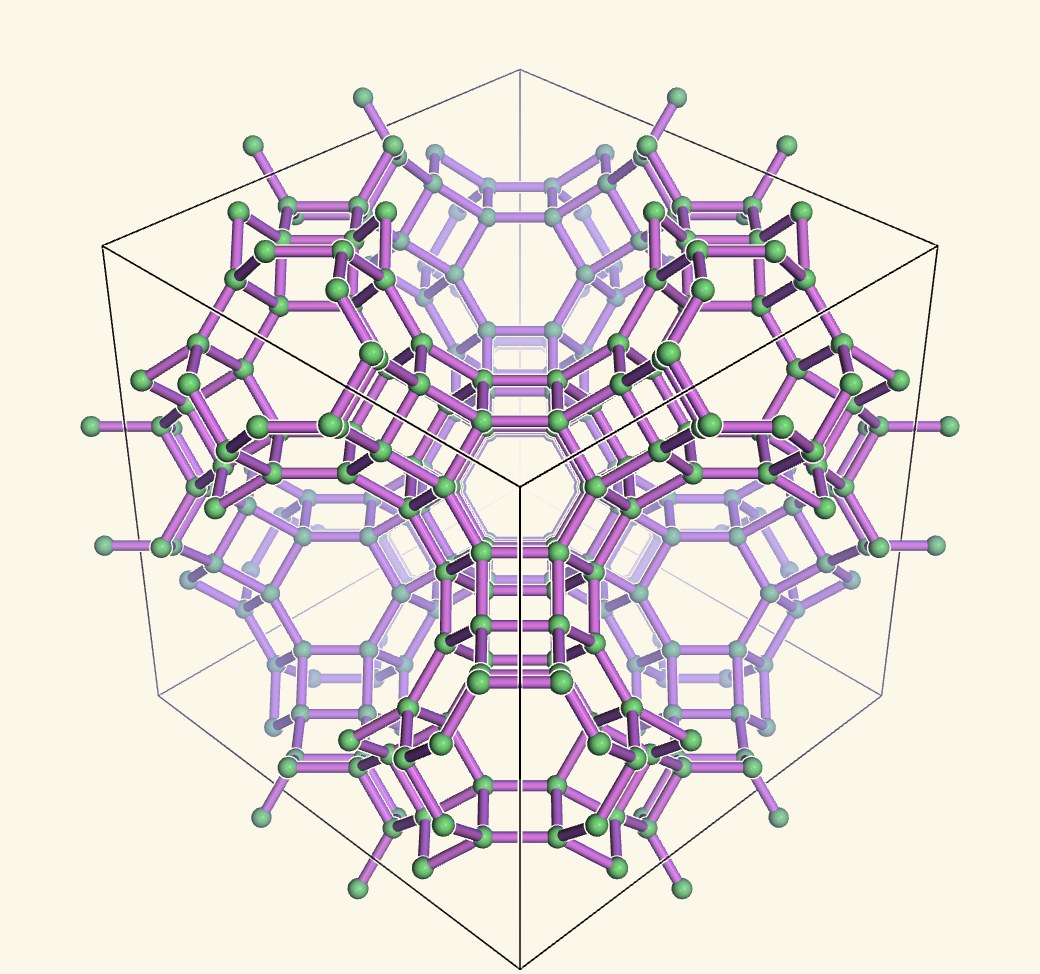
\includegraphics[height=3in]{fau-net-new}

    Adding bonds (or ligands) yields a periodic graph or {\em net}.
  \end{center}
\end{frame}

\begin{frame}
  \begin{center}
    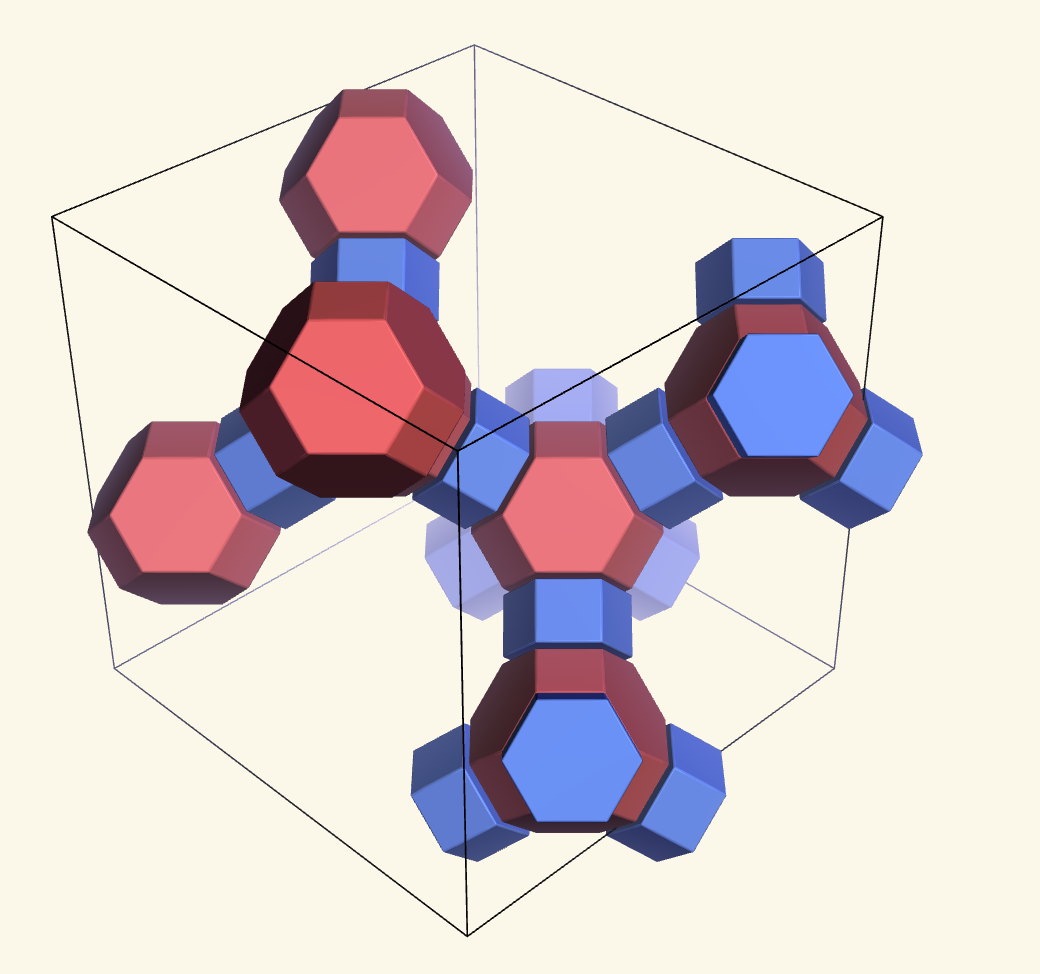
\includegraphics[height=3in]{fau-cages-new}

    Even richer structure from examining the cycle space.
  \end{center}
\end{frame}

\begin{frame}
  \begin{center}
    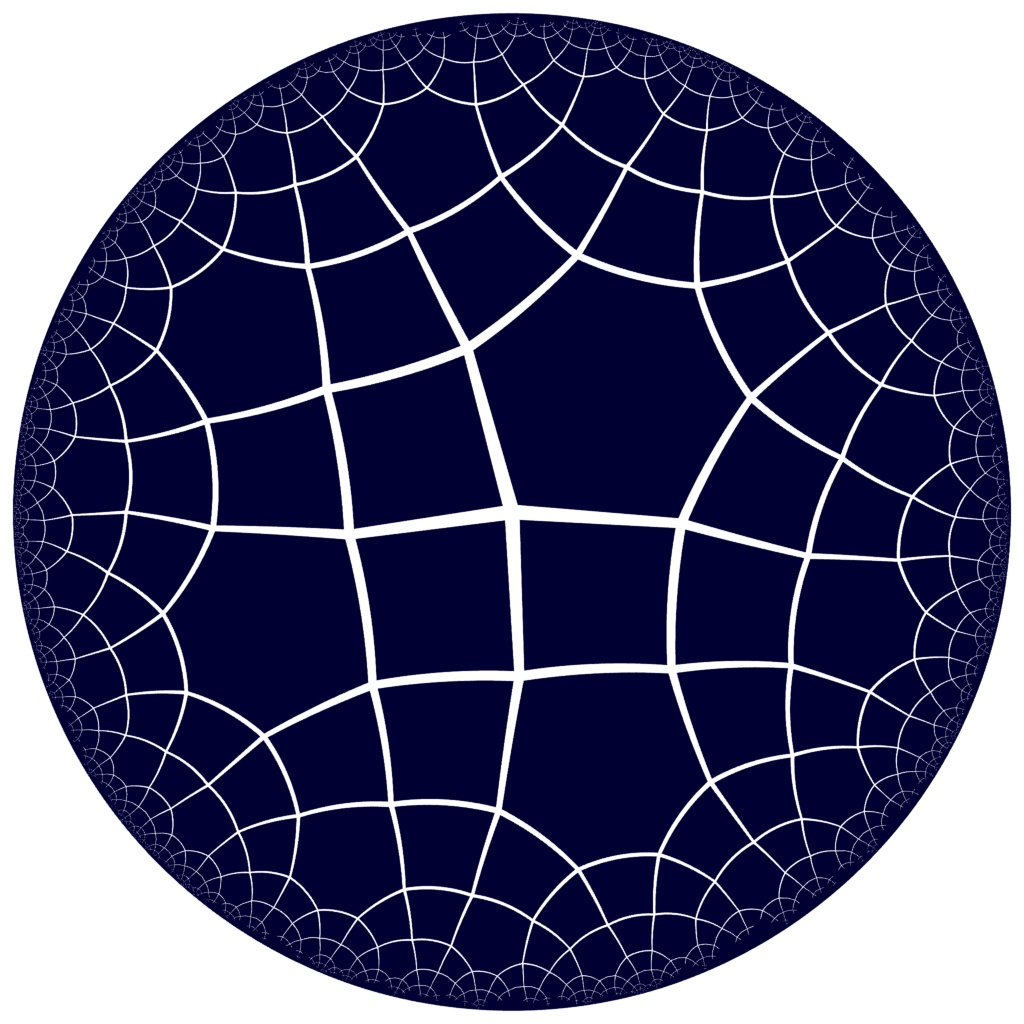
\includegraphics[height=3in]{hqc0576}

    Even richer structure from examining the cycle space.
  \end{center}
\end{frame}

\begin{frame}
  \begin{center}
    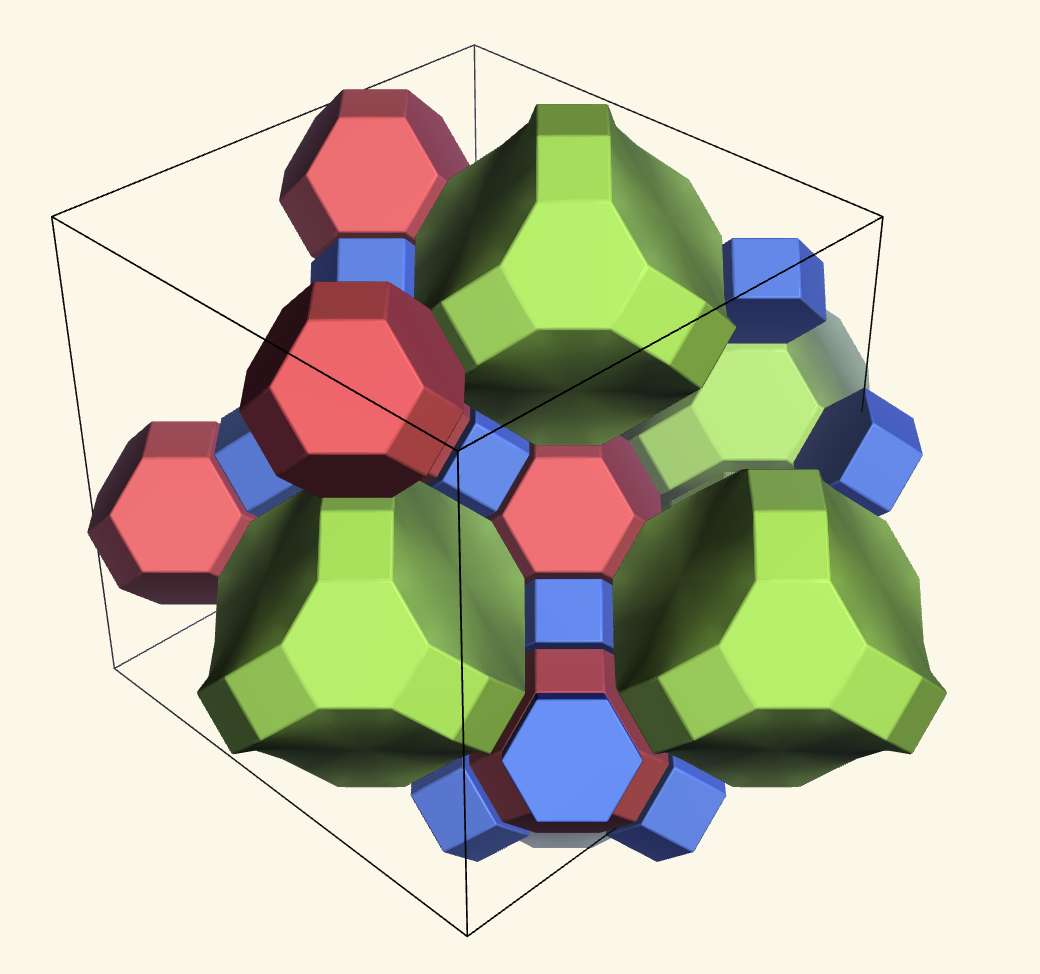
\includegraphics[height=3in]{fau-tiling-new}

    Even richer structure from examining the cycle space.
  \end{center}
\end{frame}

\begin{frame}
  \begin{center}
    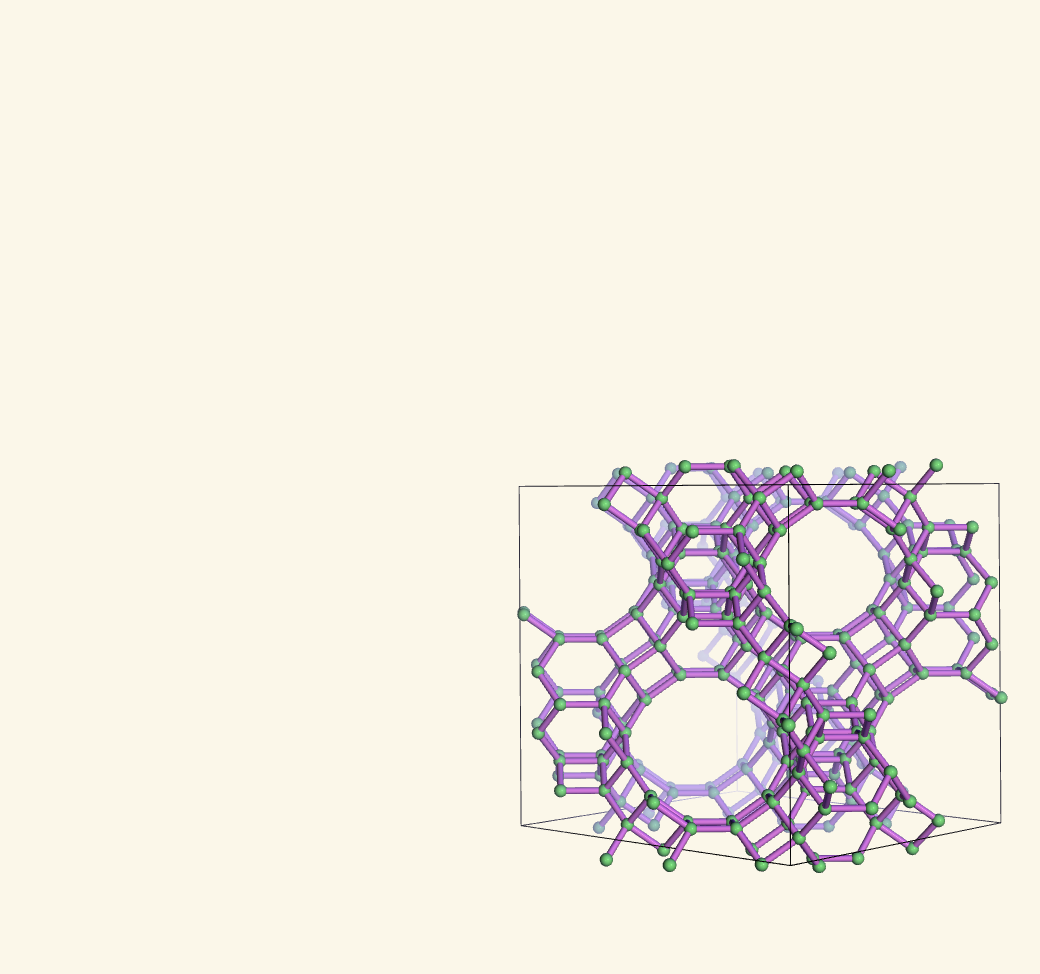
\includegraphics[height=3in]{fau-111}

    A {\em net} is a (3-) connected, locally finite periodic graph.
  \end{center}
\end{frame}

\begin{frame}
  \begin{center}
    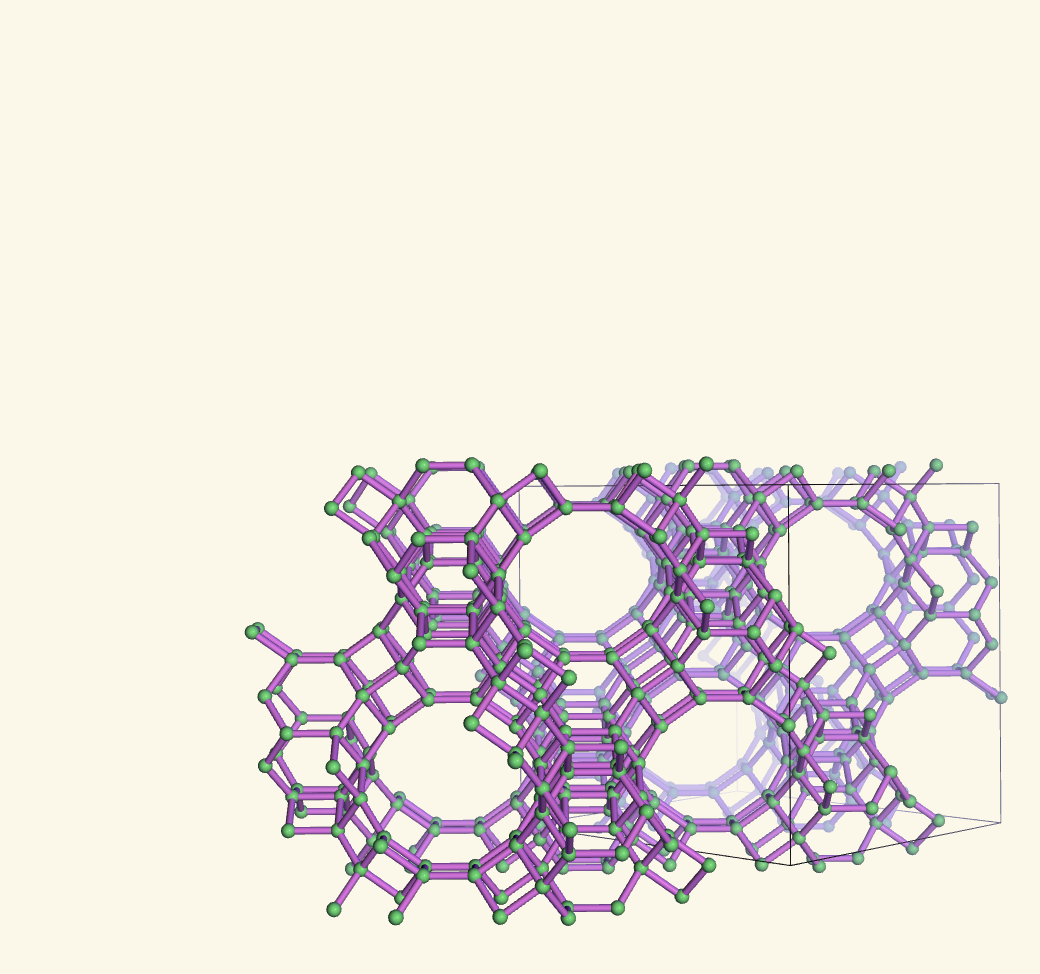
\includegraphics[height=3in]{fau-211}

    A {\em net} is a (3-) connected, locally finite periodic graph.
  \end{center}
\end{frame}

\begin{frame}
  \begin{center}
    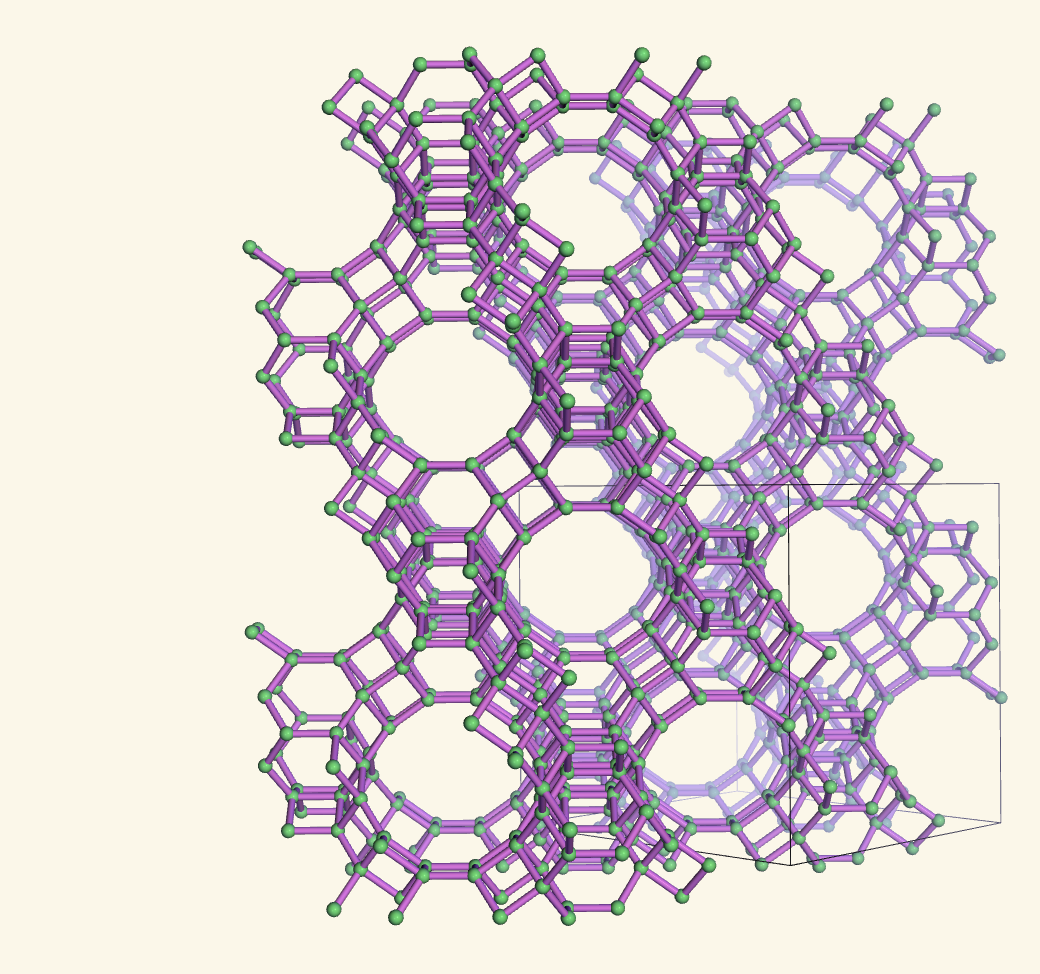
\includegraphics[height=3in]{fau-221}

    A {\em net} is a (3-) connected, locally finite periodic graph.
  \end{center}
\end{frame}

\begin{frame}
  \begin{center}
    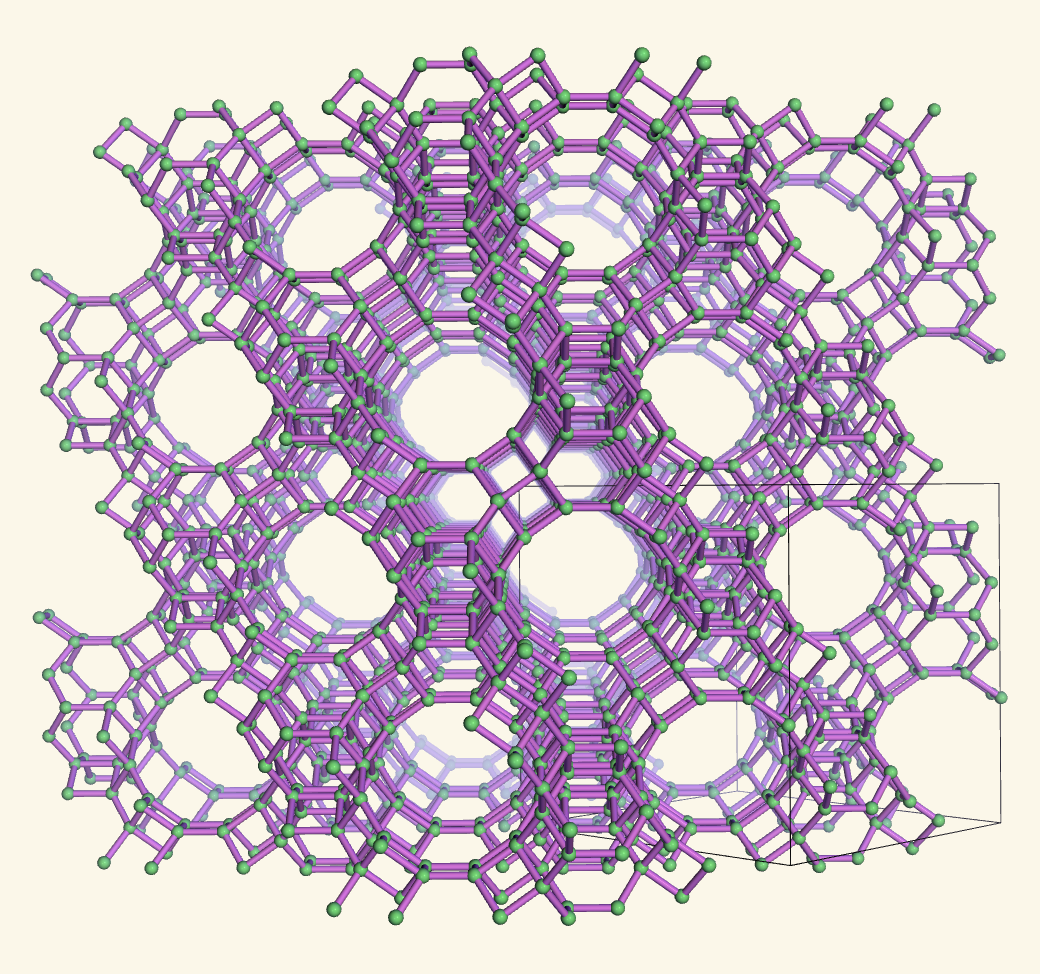
\includegraphics[height=3in]{fau-222}

    A {\em net} is a (3-) connected, locally finite periodic graph.
  \end{center}
\end{frame}

\begin{frame}
  \begin{center}
    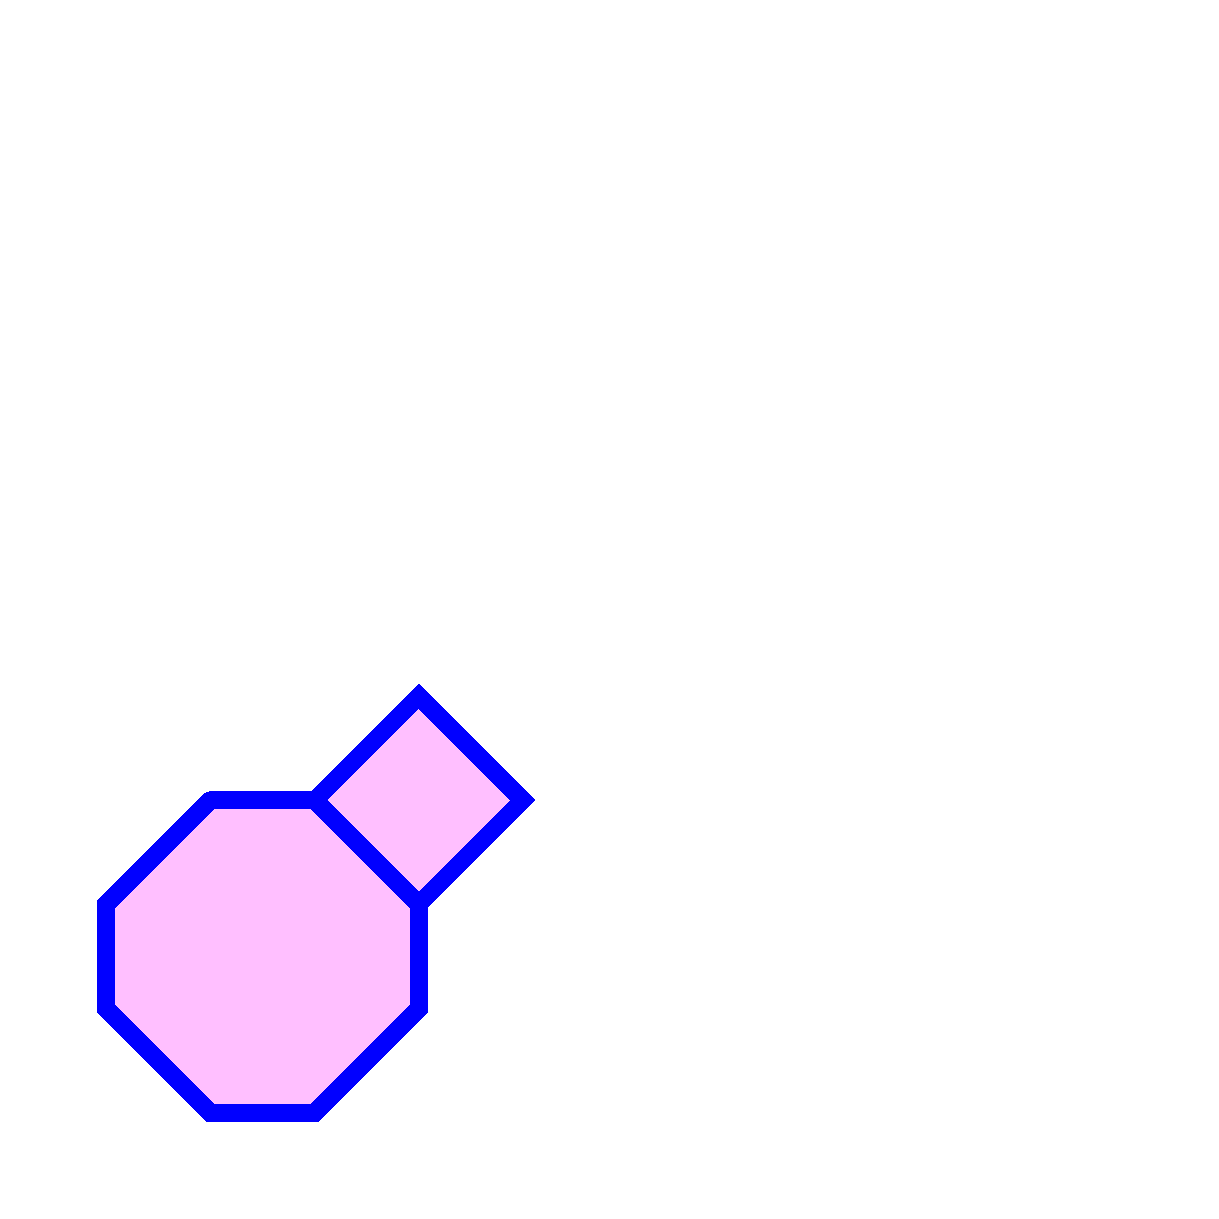
\includegraphics[width=3in]{periodic1}

    A 2-dimensional net, which here also defines a tiling.
  \end{center}
\end{frame}

\begin{frame}
  \begin{center}
    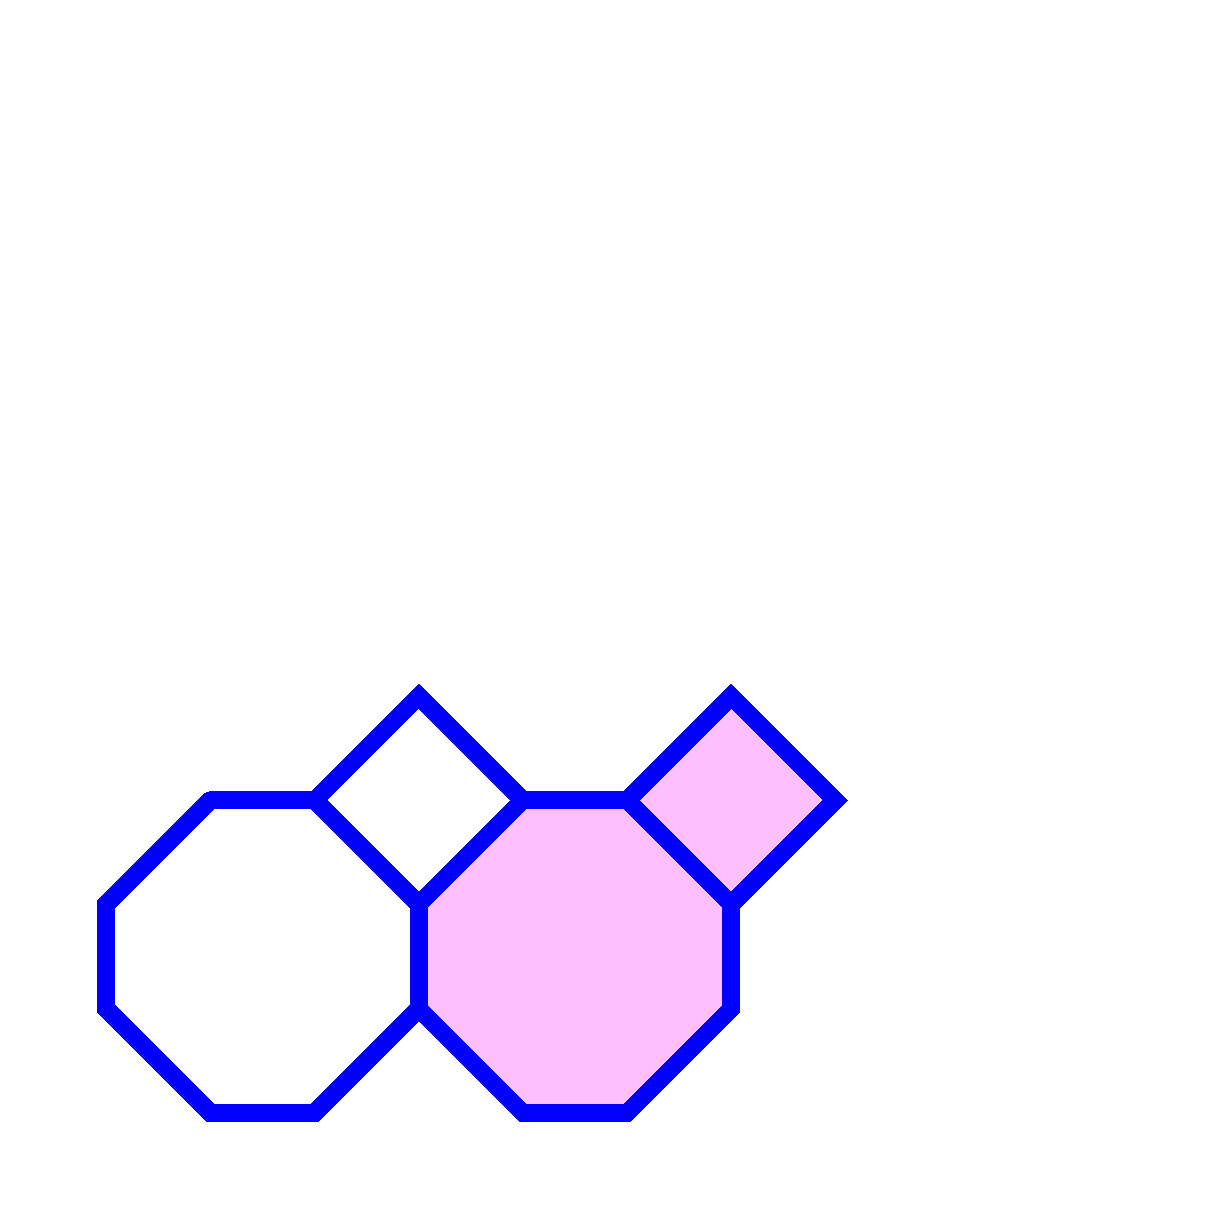
\includegraphics[width=3in]{periodic2}

    A 2-dimensional net, which here also defines a tiling.
  \end{center}
\end{frame}

\begin{frame}
  \begin{center}
    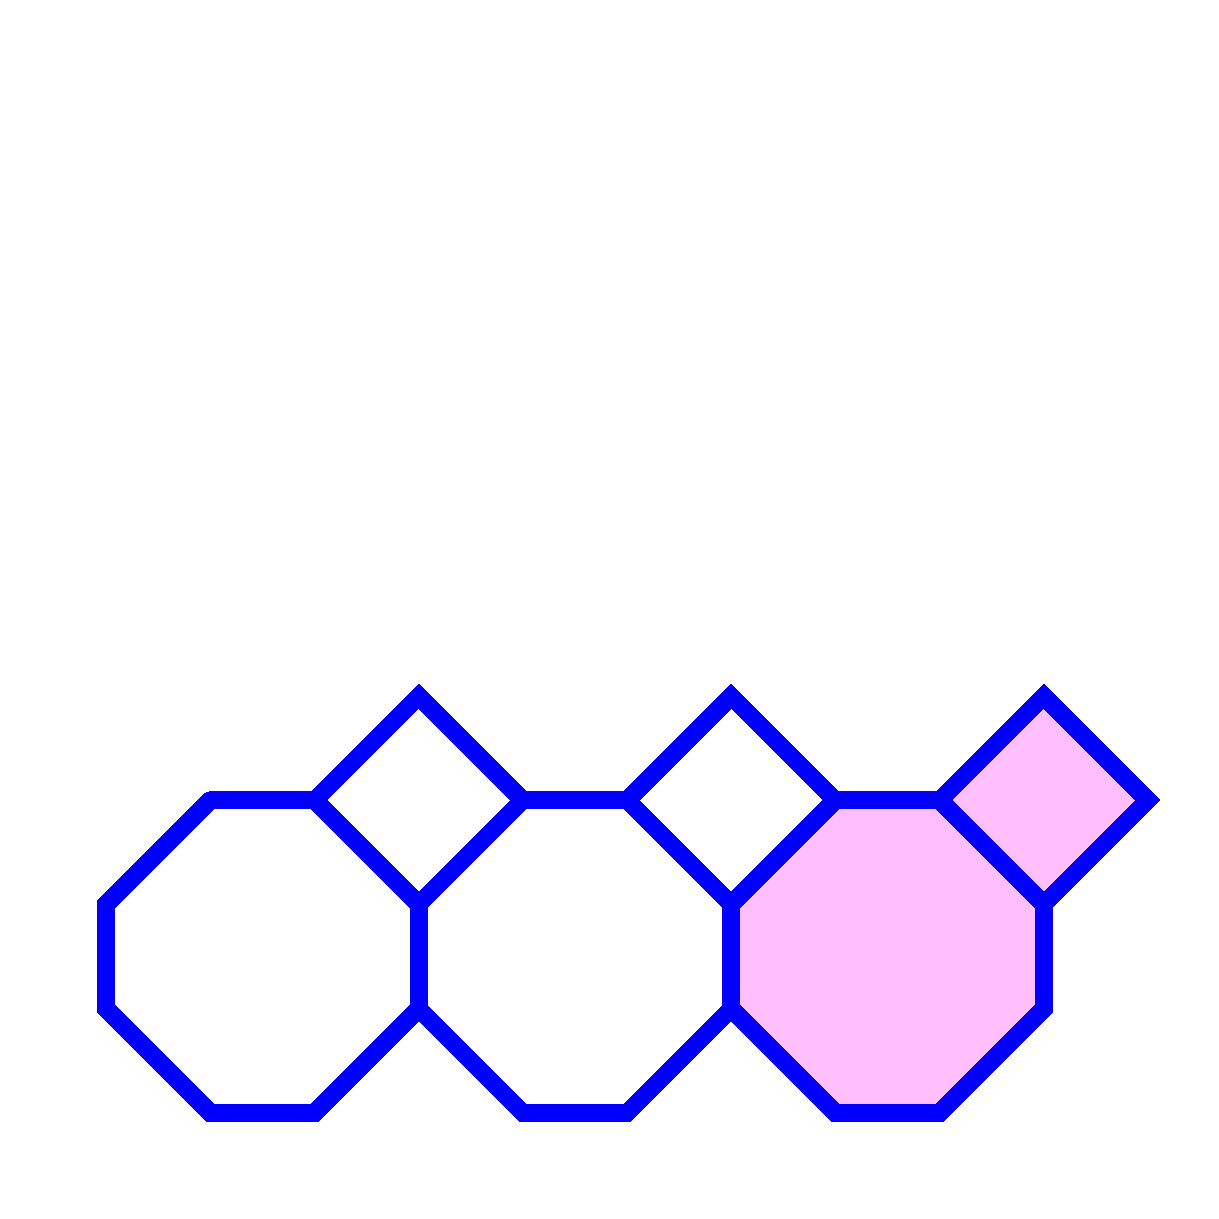
\includegraphics[width=3in]{periodic3}

    A 2-dimensional net, which here also defines a tiling.
  \end{center}
\end{frame}

\begin{frame}
  \begin{center}
    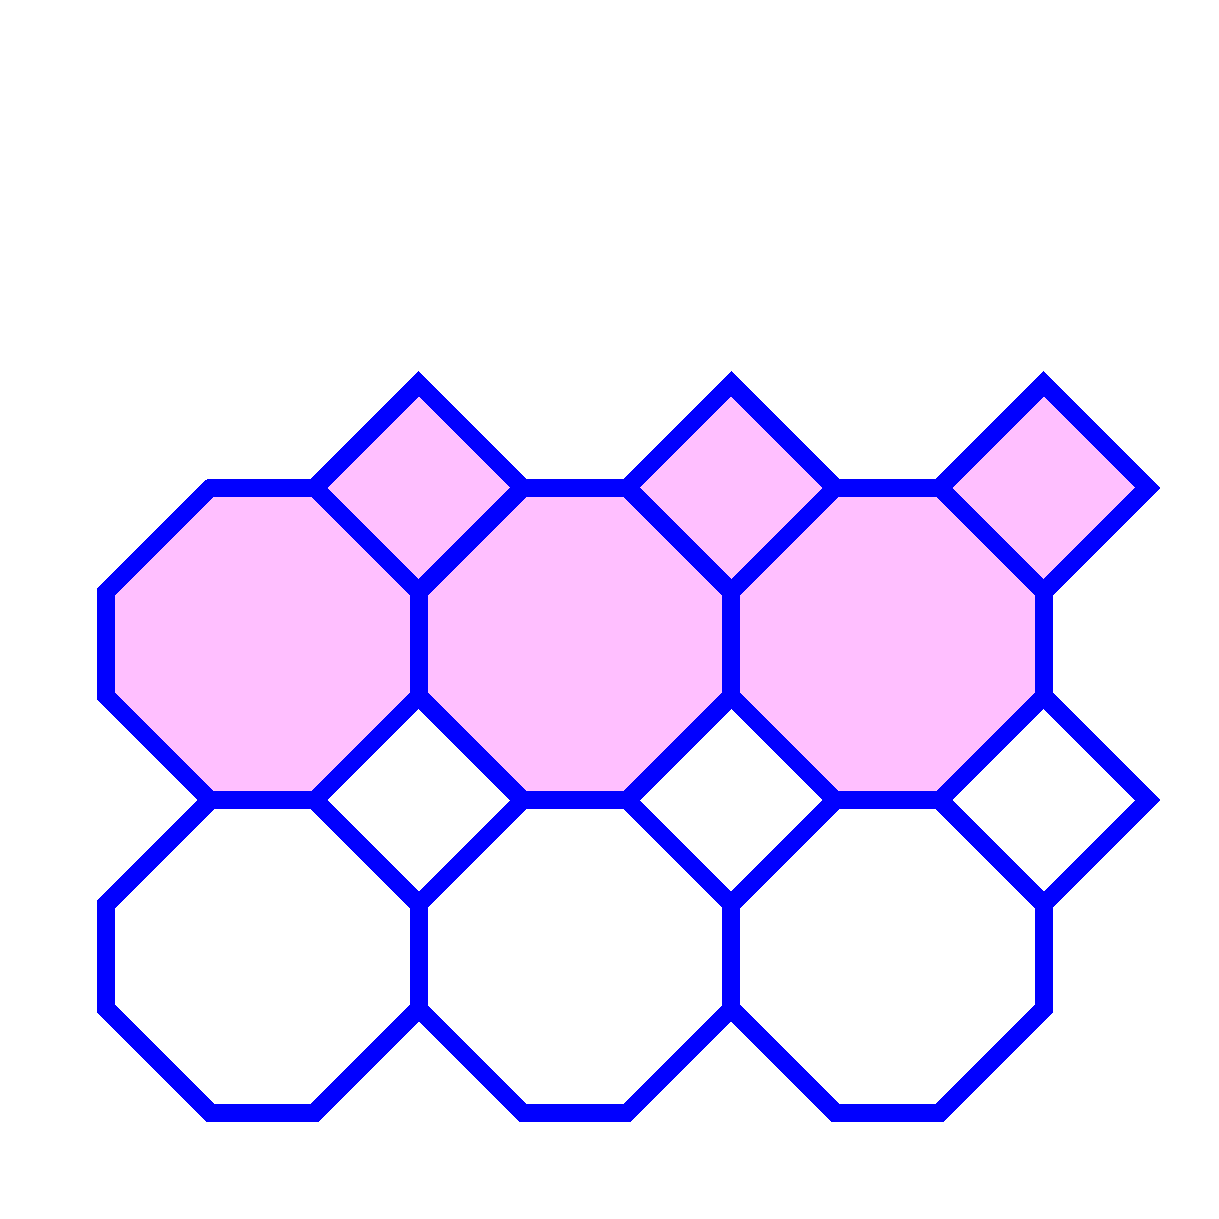
\includegraphics[width=3in]{periodic4}

    A 2-dimensional net, which here also defines a tiling.
  \end{center}
\end{frame}

\begin{frame}
  \begin{center}
    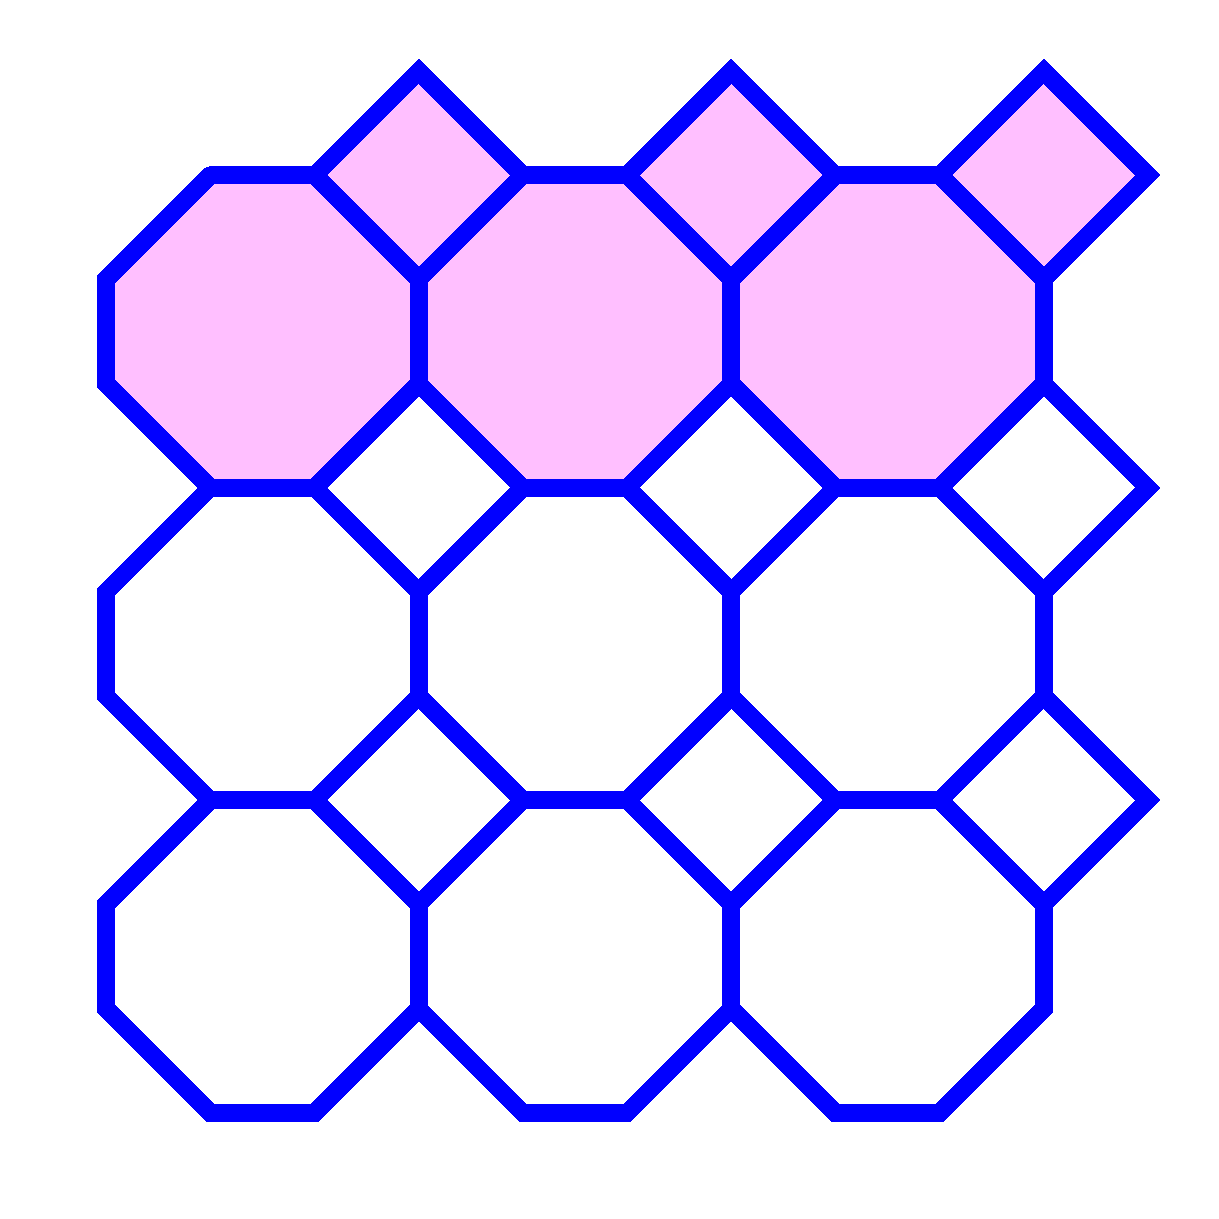
\includegraphics[width=3in]{periodic5}

    A 2-dimensional net, which here also defines a tiling.
  \end{center}
\end{frame}


\section{Crystallographic groups}

\begin{frame}
  \begin{center}
    A {\em crystallographic (space) group\/} is\\
    a discrete group of motions in euclidean space\\
    with a bounded fundamental domain.

    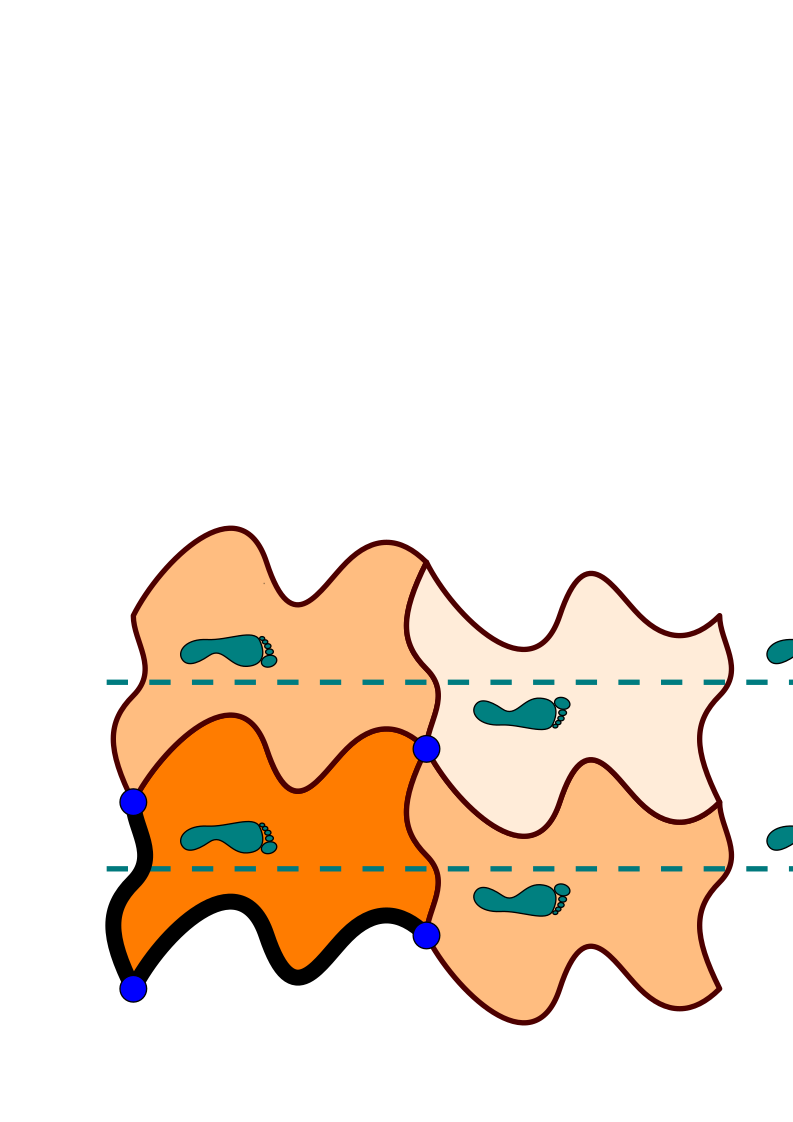
\includegraphics[width=1.7in]{heesch-TGTG}
    \qquad
    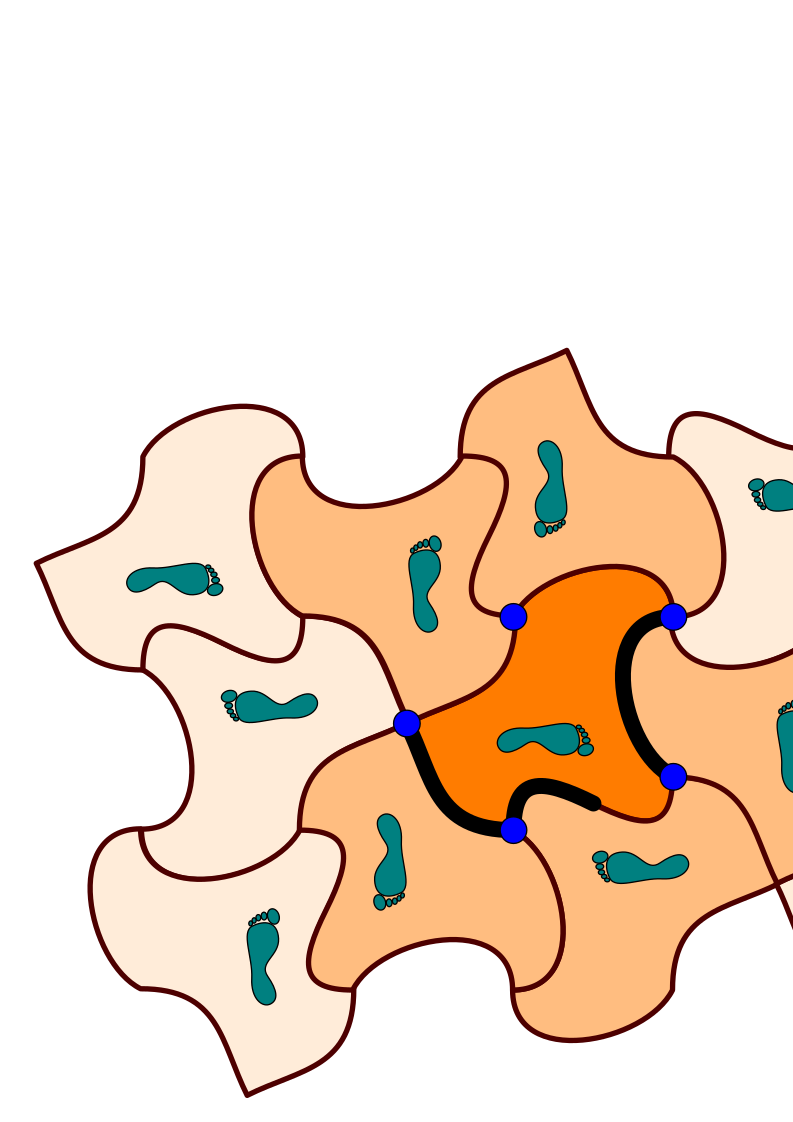
\includegraphics[width=1.7in]{heesch-C4C4C4C4C}

    Crystallographic groups are just the ones that generate\\
    unbounded, discrete point patterns.
  \end{center}
\end{frame}


\section{Tutte's barycentric embedding}

\begin{frame}
  \begin{center}
    Tutte's idea for drawing graphs ``nicely'':

    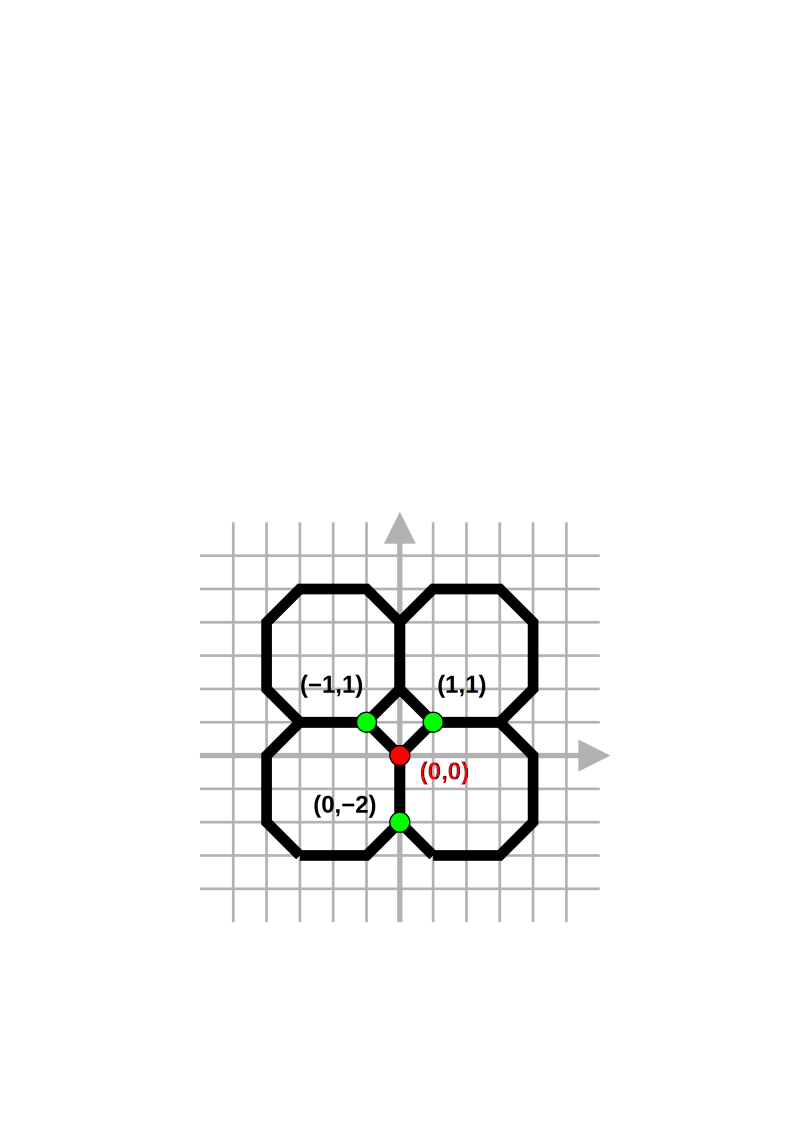
\includegraphics[width=2in]{equilibrium1}

    Place a vertex $v$ in the {\em barycenter} of its neighbors:
    \[
    \sum_{w\in Neighbors(v)} position(w)-position(v) = 0
    \]
  \end{center}
\end{frame}

\begin{frame}
  \begin{center}
    For finite graphs, prescribe a convex outer face.

    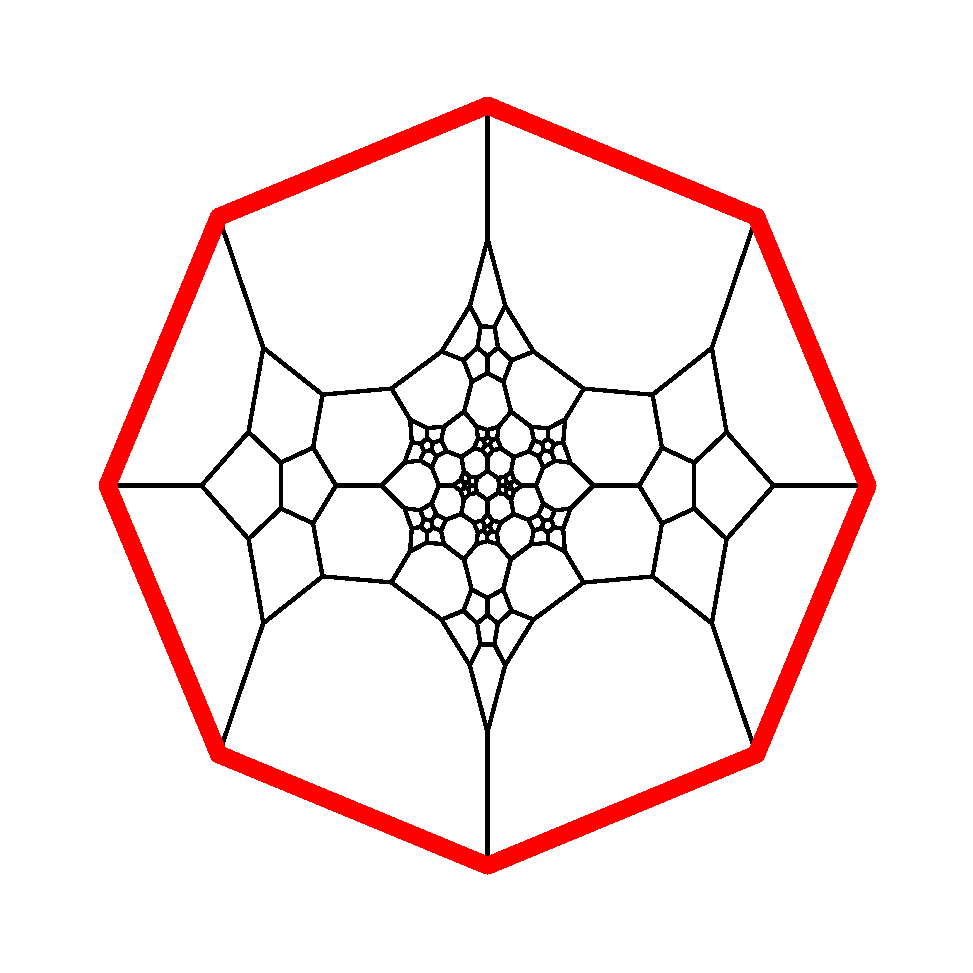
\includegraphics[width=2.5in]{schlegel2}\\
    For polyhedral graphs, this ensures convex drawings.\\
    ({\em How to draw a graph,} W.\ T.\ Tutte 1963.)
  \end{center}
\end{frame}

\begin{frame}
  \begin{center}
    For periodic graphs, prescribe a vertex lattice.

    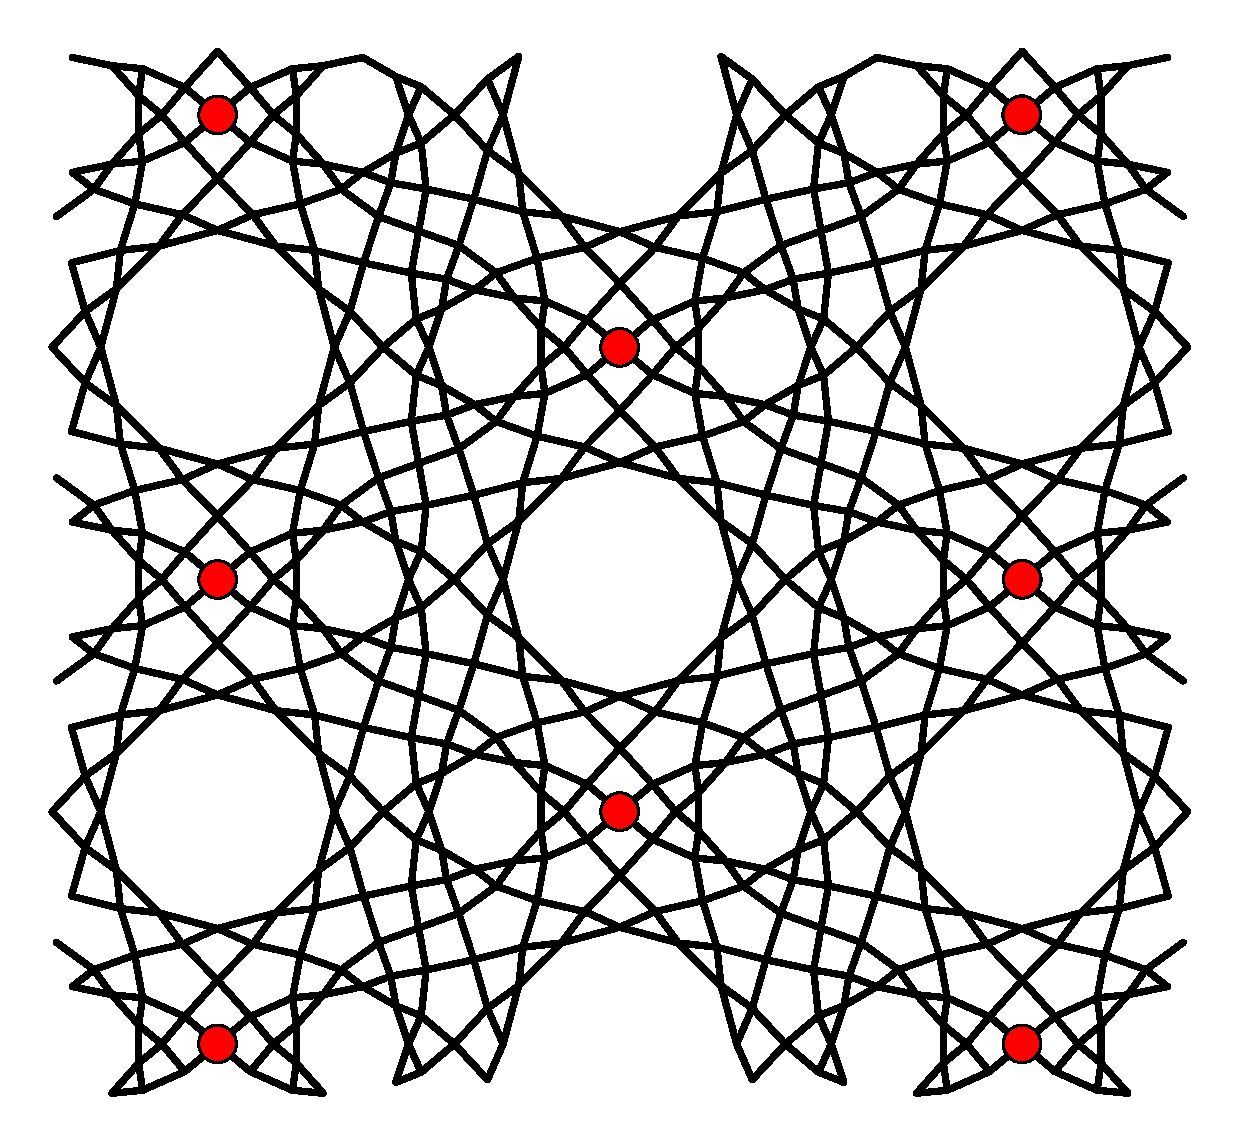
\includegraphics[width=2.5in]{al-equilibrium}

    The solution is then unique, so all periodic barycentric placements are
    the same up to affine transformations.
  \end{center}
\end{frame}


\section{Unstable nets}

\begin{frame}
  \begin{center}
    An {\em unstable} net is one with\\
    colliding barycentric vertex positions.

    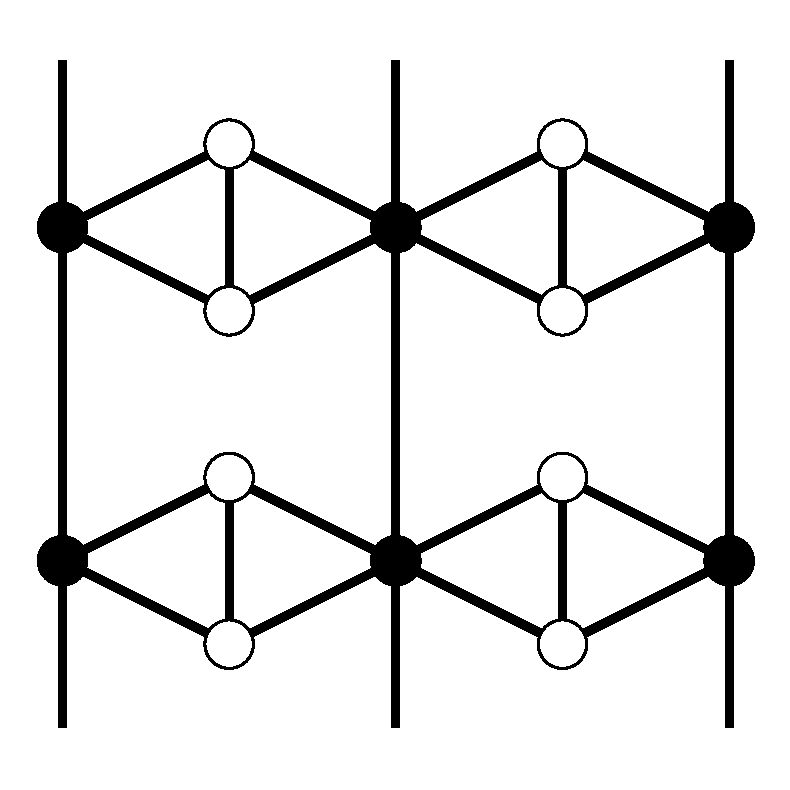
\includegraphics[width=1.1in]{unstable}
    \quad
    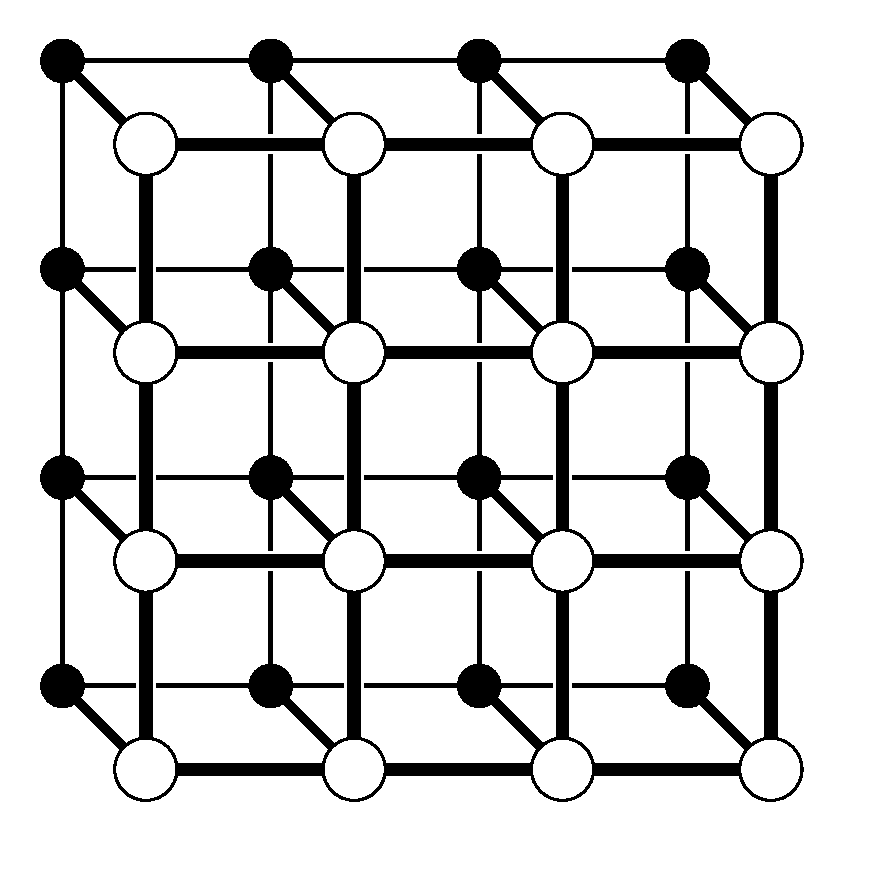
\includegraphics[width=1.1in]{ladder}
    \quad
    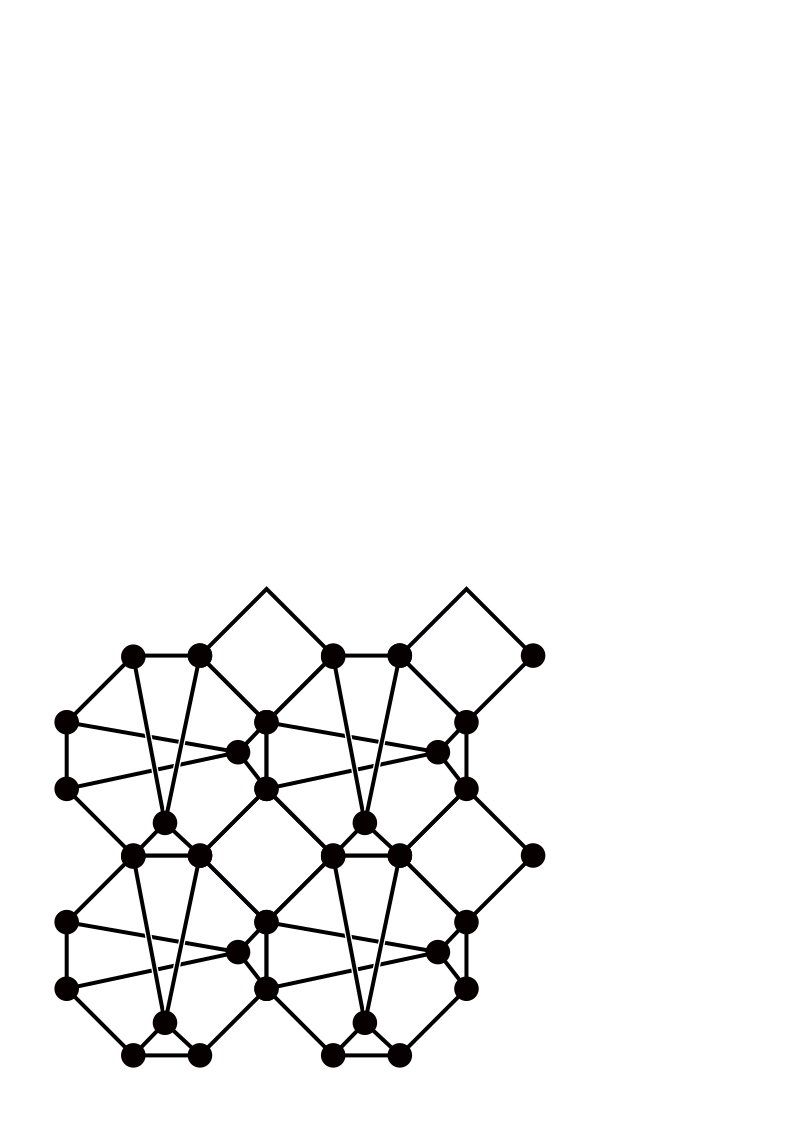
\includegraphics[width=1.1in]{collision}

    Two non-crystallographic and one crystallographic net,\\
    all unstable.

    But can non-crystallographic nets be stable?
  \end{center}
\end{frame}


\end{document}
